\documentclass[11pt,a4paper]{article}

\usepackage[margin=23mm,top=25mm,bottom=24mm,headheight=14pt]{geometry}
\usepackage[T1]{fontenc}
\usepackage{newtxtext,newtxmath}
\usepackage{microtype}
\usepackage{graphicx}
\usepackage{booktabs}
\usepackage{tabularx}
\usepackage{array}
\usepackage{multirow}
\usepackage{threeparttable}
\usepackage{enumitem}
\usepackage{xcolor}
\usepackage{caption}
\usepackage{setspace}
\usepackage{fancyhdr}
\usepackage{titlesec}
\let\openbox\relax % avoid clash between newtxmath and amsthm
\usepackage{amsthm}
\usepackage[round,authoryear]{natbib}
\usepackage[hidelinks]{hyperref}
\usepackage[nameinlink,noabbrev]{cleveref}

\graphicspath{{../reports/figures/}{reports/figures/}{figures/}}
\setstretch{1.02}
\setlength{\parindent}{1.2em}
\setlength{\parskip}{0pt}
\setlength{\tabcolsep}{4.5pt}
\setlength{\emergencystretch}{2.5em}
\renewcommand{\arraystretch}{1.1}

\hypersetup{
  pdftitle={Causal Structure Discovery via a Self-Implemented FCI+ Algorithm: A Case Study on the Tennessee STAR Project},
  pdfauthor={Yicheng Qi},
  pdfsubject={FCI, FCI+, PAG learning, Tennessee STAR, causal discovery},
  pdfkeywords={causal discovery, FCI, FCI+, PAG, latent confounding, Tennessee STAR}
}

\pagestyle{fancy}
\fancyhf{}
\fancyhead[L]{\small FCI\textsuperscript{+} and Tennessee STAR --- Final Report}
\fancyhead[R]{\small Yicheng Qi}
\fancyfoot[C]{\thepage}
\renewcommand{\headrulewidth}{0.4pt}

% Paper-style centred section headings, left-aligned bold subsections.
\titlespacing*{\section}{0pt}{1.6ex plus .4ex}{0.8ex}
\titlespacing*{\subsection}{0pt}{1.3ex plus .3ex}{0.5ex}
\titleformat{\section}{\large\bfseries\centering}{\thesection}{0.5em}{}
\titleformat{\subsection}{\normalsize\bfseries}{\thesubsection}{0.5em}{}

\captionsetup{font=small,labelfont=bf,justification=justified,
  singlelinecheck=false,skip=4pt}

\theoremstyle{definition}
\newtheorem{definition}{Definition}
\newtheorem{theorem}{Theorem}

\newcolumntype{Y}{>{\raggedright\arraybackslash}X}
\newcommand{\FCIplus}{FCI\textsuperscript{+}}
\newcommand{\code}[1]{\texttt{#1}}
% Permits a line break inside a long typewriter token without a hyphen.
\newcommand{\brk}{\discretionary{}{}{}}

\begin{document}

\pagenumbering{gobble}
\begin{titlepage}
\centering
\vspace*{1.6cm}
{\large Imperial College London\par}
\vspace{0.2cm}
{\large Department of Earth Science and Engineering\par}
\vspace{0.2cm}
{\large MSc in Applied Computational Science and Engineering\par}
\vspace{0.2cm}
{\large Individual Research Project\par}
\vspace{1.8cm}
{\LARGE\bfseries Causal Structure Discovery via a\\[0.35ex]
Self-Implemented \FCIplus{} Algorithm:\par}
\vspace{0.45cm}
{\Large A Case Study on the Tennessee STAR Project\par}
\vspace{1.6cm}
{\large\textbf{Author:} Yicheng Qi\par}
\vspace{0.3cm}
{\large\textbf{Project code:} p-anli-051\par}
\vspace{0.9cm}
{\large\textbf{Main supervisor:} Ang Li\par}
\vspace{0.12cm}
{\normalsize Florida State University \quad\textbar\quad \code{angli@cs.fsu.edu}\par}
\vspace{0.5cm}
{\large\textbf{Second supervisor:} Adriana Paluszny\par}
\vspace{0.12cm}
{\normalsize Imperial College London \quad\textbar\quad \code{apaluszn@imperial.ac.uk}\par}
\vspace{0.9cm}
{\normalsize\textbf{IRP repository:}\par}
\vspace{0.12cm}
{\normalsize\url{https://github.com/ese-ada-lovelace-2025/irp-yq225}\par}
\vfill
{\large August 2026\par}
\end{titlepage}

\pagenumbering{arabic}

\begin{abstract}
\noindent
This project develops an auditable, independent implementation of FCI and
\FCIplus{}, validates both algorithms, and applies them to the Tennessee STAR
class-size experiment. FCI learns Partial Ancestral Graphs (PAGs) under latent
confounding and selection, but its Possible-D-SEP search is expensive;
\FCIplus{} has a polynomial conditional-independence (CI) query bound for
sparse graphs. The resulting fully typed Python package contains both
paper-aligned schedules and structured decision traces, with no
causal-discovery dependency. Validation combines 367 automated tests, three
exact m-separation targets, a 15-run known-truth benchmark, and differential
comparisons with causal-learn and R \code{pcalg}. Robust \FCIplus{} attains
mean skeleton F1 0.985 and endpoint accuracy 0.840, versus 0.977 and 0.737 for
paper-profile FCI. In 6,325 STAR kindergarten-cohort students, small classes
show a 13.90-point observed kindergarten advantage (school-cluster 95\%
interval 5.21--22.07), whereas aide contrasts are near zero. This is not an
identified treatment effect because analysed outcomes are post-assignment
selected. Across methods, skeleton relations are more defensible than several
order-, threshold-, or chronology-sensitive endpoints; no learned PAG
identifies a unique DAG or effect magnitude.
\end{abstract}

\section{Introduction}
\label{sec:introduction}

\paragraph{Problem description.}
Many empirical studies ask causal questions where not every common cause has
been measured: family background, institutional selection, and administrative
recording generate dependence that no causally sufficient DAG over the
recorded columns represents honestly, and fitting one anyway turns
uncertainty into unjustified arrows. FCI was designed for this setting: under
causal Markov, faithfulness, and appropriate sampling assumptions, it learns
from conditional-independence (CI) information a Partial Ancestral Graph
(PAG) that remains valid under latent confounding and selection
\citep{spirtes2000causation,richardson2002ancestral,glymour2019review}, at
the price of an expensive Possible-D-SEP search and endpoint ambiguity;
\citet{claassen2013learning} prove a polynomial worst-case CI-query bound for
sparse graphs of fixed maximum degree \(k\).

The research problem is twofold: can FCI and \FCIplus{} be reimplemented
faithfully and verifiably from their primary sources, and what can such an
implementation legitimately conclude from a real randomized educational study
--- the Tennessee STAR class-size experiment --- whose observed data are
shaped by attrition and selection?

\paragraph{Significance.}
Public FCI-family tools typically return a finished graph with little
visibility into why each endpoint was oriented; among the interfaces checked
in \cref{sec:background}, none exposes a Python Claassen \FCIplus{} with
paper-profile control and a structured audit trail. An
implementation whose every mark traces to recorded CI decisions serves
applied researchers defending structural claims, methodologists needing a
typed reference for differential testing, and instructors separating
design-based from discovery evidence. Substantively, STAR remains a
canonical evidence source on class size, and selective attrition in
longitudinal experiments is a live methodological concern.

\paragraph{Objectives and contributions.}
Four measurable objectives respond directly to the auditability and
finite-sample gaps above; each also defines a project contribution.

\begin{description}[leftmargin=2.1em,itemsep=0.1em,topsep=0.2em,
  font=\normalfont\bfseries]
\item[O1/C1.] \emph{Implement source-faithful algorithms.} Success requires
separate paper profiles whose stages map to primary-source concepts, explicit
PAG endpoint semantics, typed public APIs, and no causal-discovery dependency.
The delivered 9,559-line, 38-module package supplies five CI tests, ordered
Possible-D-SEP, complete Algorithm~2 stages, and five orientation schedules.
\item[O2/C2.] \emph{Verify and validate.} Success requires exact recovery of
all pre-specified oracle targets, finite-sample accuracy reporting, and a clean
automated test matrix. The apparatus comprises an exact MAG m-separation
oracle, three published-structure targets, 15 known-truth runs, and 367 tests
under strict typing on Python 3.9--3.13.
\item[O3/C3.] \emph{Position against established software.} Success requires
matched-input comparisons with disclosed interface mismatches, using skeleton,
endpoint, runtime, and CI-query metrics. Executed causal-learn and R
\code{pcalg} runners provide this evidence.
\item[O4/C4.] \emph{Deliver a defensible STAR application.} Success requires
independent R replication plus school-cluster bootstrap, cyclic-order,
chronology, and sensitivity audits, with conclusions promoted only through a
pre-specified evidence hierarchy.
\end{description}

C1 and C4 are deliberately separated: the algorithm stays reusable and
domain-neutral, while the application states its own coding, selection,
clustering, and interpretation decisions.

These objectives answer one overarching question: can source-faithful FCI and
\FCIplus{} be implemented and validated well enough to support bounded,
transparent structural claims on STAR? \Cref{sec:background} establishes the
source and software gap; \cref{sec:method,sec:results} test O1--O4;
\cref{sec:interpretation,sec:conclusions} distinguish supported conclusions
from exploratory patterns. Controlled evidence precedes the application, so a
real-data pattern never serves as evidence of algorithm fidelity.

\section{Preliminaries and Related Work}
\label{sec:background}

\subsection{Graphs, assumptions, and PAGs}

Constraint-based discovery begins from statements \(X \perp Y \mid Z\) over
observed variables \(V\), with latent variables \(L\) and selection variables
\(S\) possibly present. The \emph{causal Markov condition} states that
graphical separation implies conditional independence; \emph{faithfulness}
states that observed independences arise from separation rather than exact
cancellation. Separation in a DAG is d-separation:

\begin{definition}[d-separation]
A path \(p\) is blocked by a node set \(Z\) if and only if \(p\) contains a
chain or fork whose middle node is in \(Z\), or a collider whose middle node
is neither in \(Z\) nor an ancestor of \(Z\). If \(Z\) blocks every path
between \(X\) and \(Y\), they are d-separated given \(Z\)
\citep{pearl2009causality}.
\end{definition}

Under causal sufficiency these assumptions support DAG methods such as PC.
Otherwise the appropriate observed-variable object is a maximal ancestral
graph (MAG) \citep{richardson2002ancestral}: marginalising \(L\) and
conditioning on \(S\) induce directed, bidirected, and undirected relations,
and every missing MAG edge corresponds to an \emph{m-separation}, the
generalisation of d-separation to mixed ancestral graphs and the criterion
used by this project's exact oracle. Because different MAGs can encode the
same independence model, the identifiable output is a PAG, recording exactly
the endpoint features shared by one Markov equivalence class
\citep{zhang2008completeness}.

Each PAG adjacency carries two endpoint marks: a circle leaves ancestry
unresolved, an arrowhead at \(Y\) excludes \(Y\) as an ancestor of \(X\), a
tail asserts ancestry in every represented MAG, a bidirected edge is
compatible with latent confounding without identifying a unique latent
variable, and undirected edges reflect selection structure. An adjacency says
only that the tested sets failed to separate the pair; neither an adjacency
nor an endpoint alone identifies a structural coefficient, an adjustment set,
or an interventional contrast \citep{pearl2009causality}. Sample CI tests are
error-prone, so exact-oracle recovery isolates graph logic rather than
finite-sample accuracy. Among the discovery families reviewed by
\citet{glymour2019review}, score-based search (such as GES) and standard
functional causal models (such as LiNGAM) assume causal sufficiency, so the
constraint-based FCI family is the appropriate class when latent confounding
and selection must be represented.

\subsection{Standard FCI and its historical boundary}

FCI does not require that all common causes of measured variables are
measured \citep[Ch.~6]{spirtes2000causation}. A PC-style search removes
\(X - Y\) when some subset of current neighbours separates the pair, but with
latent variables a separable pair may stay adjacent: a necessary separator
can contain a node no longer adjacent to either endpoint. The book introduces
D-SEP to characterise where an observed separator can reside and, since
D-SEP is not computable from a partial graph, an observable superset:

\begin{definition}[Possible-D-SEP]
For an ordered pair \((A,B)\) in a partially oriented graph, a node
\(V \neq A\) belongs to \(\mathrm{Possible\text{-}D\text{-}SEP}(A,B)\) if
some path from \(A\) to \(V\) has every internal triple either a collider or
a triangle whose middle node is not a definite noncollider
\citep{spirtes2000causation}.
\end{definition}

The construction is deliberately permissive and required \emph{separately}
from each ordered endpoint: using one direction only, or mixing pools,
changes the search contract. The full schedule: PC-style adjacency search;
initial unshielded colliders; ordered Possible-D-SEP refinement; endpoint
reset and collider reconstruction from final separators; orientation
closure. Theorem 6.4 of the source guarantees a correct \emph{partially
oriented inducing path graph} under correct population-level CI decisions
--- while the authors state they did not know whether the output was
maximally informative. Complete orientation therefore depends on the later
rules of \citet{zhang2008completeness} and is not retroactively attributed to
the 2000 source.

\subsection{\texorpdfstring{\FCIplus{}}{FCI+}: Algorithm 2}

\citet{claassen2013learning} ask whether causal discovery remains
intrinsically exponential when the observed structure is sparse. Their
central result, restated in the form used throughout this report:

\begin{theorem}[\citealp{claassen2013learning}]
Assume a constant-time exact independence oracle, a distribution faithful to
a causal DAG, and an observed-variable MAG of maximum degree at most a
constant \(k\). Then Algorithm~2 (\FCIplus{}) returns the completed PAG over
\(N\) observed variables using \(O(N^{2(k+2)})\) CI queries in the worst
case.
\end{theorem}

The claim is narrower than the paper's title: it bounds oracle queries and
does not make a statistical test exact or constant-time. A nonadjacent pair
in the true MAG can survive bounded adjacency search when every useful
separator requires a node outside the endpoint-adjacency union; such a false
adjacency is a \emph{D-sep link}. Rather than searching a large
Possible-D-SEP pool, \FCIplus{} extracts invariant non-ancestry into an
\emph{augmented skeleton} \(G^{+}\): when a known minimal independence
\(X \perp Y \mid S\) becomes dependence given \(S \cup \{A\}\) for a suitable
adjacent \(A\), an invariant arrowhead at \(A\) is supported. In \(G^{+}\), a
D-sep link \(X - Y\) appears as the middle edge of
\(U \leftrightarrow X \leftrightarrow Y \leftrightarrow V\) with \(U\),
\(V\) nonadjacent and cross-direction paths not running against an
arrowhead; the pattern only \emph{proposes} a candidate, and independence
evidence decides deletion. Conditioning sets come from the recursive
hierarchy \(\mathrm{HIE}(X, I)\), the fixed point of repeatedly adding
recorded minimal separators of members; because candidates can depend on one
another, each successful removal rebuilds the augmented skeleton and
candidate list (\cref{fig:workflow}). The arXiv supplement's abstract states
\(N^{2(k+1)}\) while its theorem and proof agree with the UAI paper's
\(N^{2(k+2)}\), a discrepancy recorded rather than harmonised. Algorithm~2
invokes complete FCI orientation rather than rederiving it, so its
completed-output claim inherits \citet{zhang2008completeness} as a
dependency.

\begin{figure}[!t]
\centering
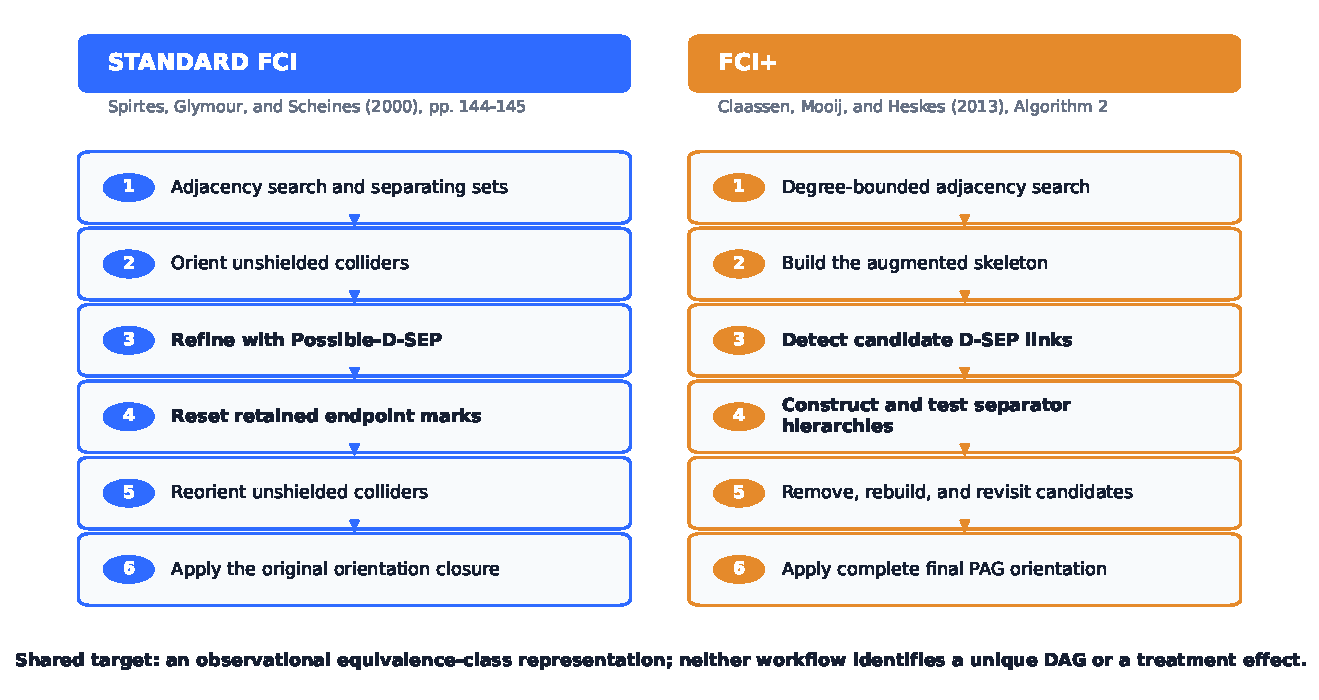
\includegraphics[width=\textwidth]{fci_fci_plus_workflow.pdf}
\caption{Source-located control-flow comparison. Standard FCI performs a
non-local Possible-D-SEP refinement; \FCIplus{} instead iterates
augmented-skeleton, candidate D-sep-link, hierarchy, and minimal-separator
stages before invoking final orientation. The robust application profile of
\cref{sec:method} changes finite-sample policy, not the definition of
Algorithm~2.}
\label{fig:workflow}
\end{figure}

\subsection{What the sources do not establish}

Neither source guarantees finite-sample recovery: both theorems are
conditional on correct CI decisions. Neither identifies a unique DAG, an
adjustment set, or a treatment effect; a bidirected pattern does not name or
measure a hidden cause. The 2000 source proves no maximal orientation and no
polynomial bound; the 2013 source proves no finite-sample superiority and
nothing when \(k\) is wrong --- a user-entered bound is not evidence --- and
its authors warn that hierarchy-derived conditioning sets may be large,
reducing finite-sample power.

\subsection{Existing software}

\Cref{tab:capability} summarises the dated capability comparison: \code{pcalg}
\citep{kalisch2012pcalg} exposes both algorithms and accepts user-defined CI
tests, but its \code{fciPlus} result carries materially less separator
provenance; causal-learn \citep{causallearn2026} exposes standard FCI but no
public Claassen \FCIplus{} entry point; Tetrad \citep{tetrad2026} provides
FCI-family hybrids, none established as a drop-in Claassen \FCIplus{}, and
was checked at documentation level only (no working Java runtime). The
originality of this work is therefore not a new algorithm but a verifiable
one: paper-profile control, structured traces, separator provenance,
per-edge explanations, and stability auditing integrated in one workflow ---
an auditability improvement, not a universal accuracy or speed claim.

\begin{table}[!t]
\caption{Dated public-interface capability comparison (26 July 2026). All
four tools expose standard FCI; ``partial'' means some information is
obtainable, but not through the same integrated result contract. Tetrad is
documentation-only because no working Java runtime was available.}
\label{tab:capability}
\footnotesize
\begin{tabularx}{\textwidth}{>{\raggedright\arraybackslash}p{0.145\textwidth}
  >{\raggedright\arraybackslash}p{0.115\textwidth}
  >{\raggedright\arraybackslash}p{0.085\textwidth}
  >{\raggedright\arraybackslash}p{0.11\textwidth}
  >{\raggedright\arraybackslash}p{0.13\textwidth}Y}
\toprule
Tool & Claassen \FCIplus{} & Custom CI & Sepset provenance &
Order/bootstrap audits & Structured audit and export \\
\midrule
\code{fci\_engine} 0.1.0 & yes & yes & yes, stage named & both &
CI and orientation traces; D-SEP diagnostics; per-edge explanations;
JSON/CSV/HTML \\
\code{pcalg} 2.7-12 & yes & yes & partial & order partial &
standard-FCI sepsets; no equivalent bundled export established \\
causal-learn 0.1.4.7 & no public entry point found & named tests &
not exported & not established &
graph return; no equivalent structured trace established \\
Tetrad 7.6.10 & not established & yes & yes & partial, broader workflow &
logger and GUI facilities; not executed here \\
\bottomrule
\end{tabularx}
\end{table}

\section{Methodology}
\label{sec:method}

\subsection{Package design}

The package exposes the obligations of \cref{sec:background} as inspectable
components, separate from application policy: reusable code in
\code{src/fci\_engine}, the STAR workflow in
\code{case\_studies/tennessee\_star}, no STAR-specific choice in the
estimator. The algorithms are separate entry points with explicit paper
profiles, so a finite-sample default cannot silently stand in for the source
algorithm. \code{FCIConfig.paper()} fixes unbounded depth, immediate
deletion, first-found separators, enabled Possible-D-SEP, nonconservative
colliders, and the historical \code{spirtes\_2000} closure;
\code{FCIPlusConfig.paper(k)} requires an explicit \(k\) for both
conditioning depth and sparsity bound, disables Possible-D-SEP, and selects
the complete \code{standard} closure required by Algorithm~2's output claim.
Profiles constrain execution; they do not validate theorem assumptions ---
supplying \(k=3\) does not prove the true MAG has degree at most three.

The \code{PAG} class stores an endpoint mark at each side of every adjacency,
keeping tails, arrowheads, circles, and absence explicit. Every search uses
one \code{CITest.test(data, x, y, cond\_set)} contract, with built-in
Fisher-Z, missing-value Fisher-Z, chi-square, G-square, and kernel tests. A
cache canonicalises each query, separating the \emph{logical} CI requests
made by control flow from cache hits and executed statistics --- the
distinction relevant to a theorem counting oracle queries.

\code{FCI.fit} exposes the source stage ordering, recording Possible-D-SEP
removals with source \code{pdsep}. \code{FCIPlus.fit} deliberately does not
call Possible-D-SEP; it passes the initial skeleton to the Algorithm~2
search: augmented skeleton, bidirected witness patterns, paired endpoint
bases, hierarchy fixed points, separator testing and minimisation, graph
update, and candidate rebuild. A
diagnostics record counts candidates, revisits, hierarchy queries,
D-SEP-stage CI requests, and the maximum conditioning size --- empirical
accounting, not a mechanised proof of the bound. One dispatcher provides
five orientation schedules: \code{spirtes\_2000}, the historical closure
used by the standard-FCI paper profile; \code{standard}, the modern complete
schedule required by the \FCIplus{} paper profile; and \code{conservative},
\code{leaf}, and \code{robust}, finite-sample engineering policies
supporting no completed-PAG claim. A regression verifies that
\code{spirtes\_2000} stops before a selection-bias tail completion that
\code{standard} orients, making the historical boundary executable.
\code{FCIResult} binds the final graph to the evidence that produced it ---
configuration, separators with stage sources, logical CI counts, and named
CI and orientation traces; \code{explain\_edge} returns every decision
behind a pair, so a plotted arrow cannot detach from the profile, test,
threshold, and rule that created it.

The code base was written entirely for this project: a 9,559-line, 38-module
algorithm package; 367 tests in 44 modules (5,929 lines); a 3,052-line STAR
application with a 396-line independent R runner; and benchmark and figure
scripts --- roughly 25,300 lines in total. The
package ships \code{py.typed} and passes Ruff, strict MyPy, a wheel build,
and Pytest on Python 3.9--3.13; a full concept-to-symbol-to-test
traceability matrix is maintained in the repository's extended report. These
checks establish interface and packaging consistency, not faithfulness, true
sparsity, or any empirical causal conclusion.

The practical profile trades computation for stability: stable deletion
reduces order dependence; max-\(p\) separators spend more CI queries for
stronger independence evidence; conservative collider and tail policies
preserve circles; automatic \(\alpha\) is a documented sample-size
heuristic. Accordingly, ``paper \FCIplus{}'' is the fidelity and
query-efficiency subject; ``robust \FCIplus{}'' is the preferred application
policy, meeting the stated audit criteria while returning less-specific
endpoints --- a local preference, not a universal ranking.

\subsection{Validation and comparison design}

The strongest tests replace sample CI decisions with exact m-separation in a
known MAG, isolating search correctness from sampling error. Three
independently specified targets come from published structures: the
canonical Figure~4(b) D-SEP example of \citet{claassen2013learning}, a
latent-variable reference graph from the FCI literature, and an
orientation-rule reference graph associated with
\citet{zhang2008completeness}. Finite-sample behaviour is then tested on 15
deterministic latent-SEM cases --- five graph families, three seeds each,
2,500 observations, known oracle PAGs.

The software comparison separates execution from interface inspection: the
capability layer appears in \cref{sec:background}; the executed layer asks
what happened on identical committed data under recorded settings. The
benchmark reuses the 15 known-truth runs, every
method receiving the same numeric matrix and variable order. Fixed paper and
reference rows use Fisher-Z at \(\alpha = 0.001\); robust \FCIplus{} uses
its documented sample-size rule, which resolves to \(\alpha = 0.01\) here
--- intentional: that row evaluates the public robust policy, not a literal
Algorithm~2 reproduction. Exact F1 requires both endpoint marks to match;
semantic F1 additionally credits endpoint patterns compatible with the
target ancestral constraints; endpoint accuracy scores individual marks. The
common conversion represents each edge as an unordered pair plus two
semantic marks, never as generic directed edges. Throughout, data, order,
alpha, and CI semantics are held fixed where interfaces allow, every
mismatch is disclosed, and distinct FCI-family algorithms are never
relabelled as one.

\subsection{STAR data and panels}

The Tennessee Student/Teacher Achievement Ratio project was a large
randomized experiment in kindergarten through grade 3, assigning students
and teachers to small classes (about 13--17 students), regular classes
(about 22--25), or regular classes with a full-time aide
\citep{word1990star}; it remains a central source of evidence on class size
\citep{krueger1999experimental}. This analysis uses the official Harvard
Dataverse release \citep{achilles2008star}: 11,601 student records, 379
variables, CC0 licence, codes checked against the 146-page user guide.

Randomization already provides a stronger basis for estimating the
class-size effect than structure learning, so FCI is not used to rediscover
it. The purposes are structural: the attrition structure of grade-3
observation; the persistence of the early--later achievement adjacency; the
effect of an early post-assignment outcome's inclusion; cross-implementation
agreement; and \FCIplus{}'s search savings. The design also supplies an external audit: a
data-only PAG implying an implausible pre-treatment direction, or latent
confounding of a randomized assignment, should be reported as a discrepancy
rather than accepted literally.

The analysis covers the 6,325 students with a kindergarten class assignment
across 79 schools, arranged into three panels deliberately not pooled
because each encodes a different statistical question (\cref{tab:panels}).
All model inputs are integer-coded discrete categories: class arm, sex,
ethnicity (small source categories collapsed), free-lunch status, school
context, entry-age quantiles, binned teacher experience, and
reading-plus-mathematics scaled scores converted to achievement quartiles;
the exact numeric tables supplied to the algorithms are committed in the
repository.

\begin{table}[!t]
\caption{STAR analysis panels.}
\label{tab:panels}
\begin{tabularx}{\textwidth}{lrrY}
\toprule
Panel & Rows & Nodes & Purpose \\
\midrule
Attrition / observation & 5,744 & 9 &
Relate assignment, characteristics, context, and kindergarten achievement to
whether both grade-3 scores are observed. \\
Longitudinal achievement & 2,787 & 9 &
Study structure between kindergarten and grade-3 achievement among complete
cases while retaining early achievement. \\
Focused treatment-outcome & 2,976 & 8 &
Study the class-assignment/grade-3 relationship without allowing
kindergarten achievement, an early post-assignment outcome, to serve as a
separator. \\
\bottomrule
\end{tabularx}
\end{table}

\subsection{Discovery protocol and audits}

Before discovery, randomized-arm contrasts are computed for kindergarten
scores, grade-3 scores among students with both scores, and the probability
that both are observed, with uncertainty from 1,000 kindergarten-school
bootstrap samples; these design-based contrasts are reported separately from
discovery output.

Discovery uses the likelihood-ratio G-square test,
\(G^2 = 2 \sum_s \sum_{x,y} O_{xys} \log ( O_{xys} / E_{xys} )\), at
\(\alpha = 0.05\) --- chosen because every panel variable is an
integer-coded category, where Fisher-Z's Gaussian-linear assumptions do not
apply, at the cost of sparse contingency cells under high-order
conditioning. Standard FCI runs its unbounded paper schedule; paper
\FCIplus{} uses \(k = 3\); robust \FCIplus{} uses the practical profile
(stable skeleton, strongest separating sets, conservative colliders, robust
orientation, depth and sparsity bound 3); the independent reference is
\code{pcalg::fciPlus} with selection bias enabled and no exposed \(k\). No
temporal priors are supplied to discovery; reversals are audited after
fitting.

Alternatives were rejected for stated reasons: PC and GES impose causal
sufficiency; Fisher-Z mismatches the discrete panels; kernel CI is far more
expensive and does not solve clustered sampling; and adding temporal priors
would conceal, rather than test, chronology failures. A formal randomized
treatment-effect model is complementary to the structural question and is
therefore kept outside the discovery analysis.

Three audits probe stability: 100 school-cluster bootstrap refits per
algorithm and panel, recording each unordered adjacency's appearance
frequency (an exploratory diagnostic, not a posterior probability); a
cyclic-order audit refitting every cyclic shift of the variable list for all
profiles and the R reference; and a focused-panel sensitivity grid over
\(\alpha \in \{0.01, 0.05\}\), three versus four quantile bins, and
\(k \in \{2,3,4\}\).

A skeleton-level conclusion is promoted only when the adjacency survives
every cyclic shift with high bootstrap frequency; a directional conclusion
additionally requires invariant endpoint marks, no conflict with measurement
time or randomization, and no material reversal under sensitivity checks;
failure downgrades the claim to unresolved direction rather than deleting
the edge.

\section{Results}
\label{sec:results}

\subsection{Exact-oracle validation}

Both algorithms recover all three encoded targets, with Figure~4(b)
additionally tested under four variable orders. The Figure~4(b) MAG has six
edges (\(Z \rightarrow U\), \(Z \rightarrow V\), \(U \leftrightarrow X\),
\(V \rightarrow X\), \(U \rightarrow Y\), \(V \leftrightarrow Y\)); the
adjacency stage retains a false \(X - Y\) link although
\(X \perp Y \mid \{U,V,Z\}\), with \(Z\) adjacent to neither endpoint. The
source exhibits this separator but prints no endpoint-complete PAG, so the
completed comparison target is repository derived (\cref{fig:figure4}). Here paper-aligned standard FCI needs 102 CI
queries and \FCIplus{} 63 (a 38.2\% reduction), both returning the exact
target; the values are
frozen in \code{reports/data/\brk oracle\_validation\_summary.csv} with
target hash and separator provenance.

\begin{figure}[!t]
\centering
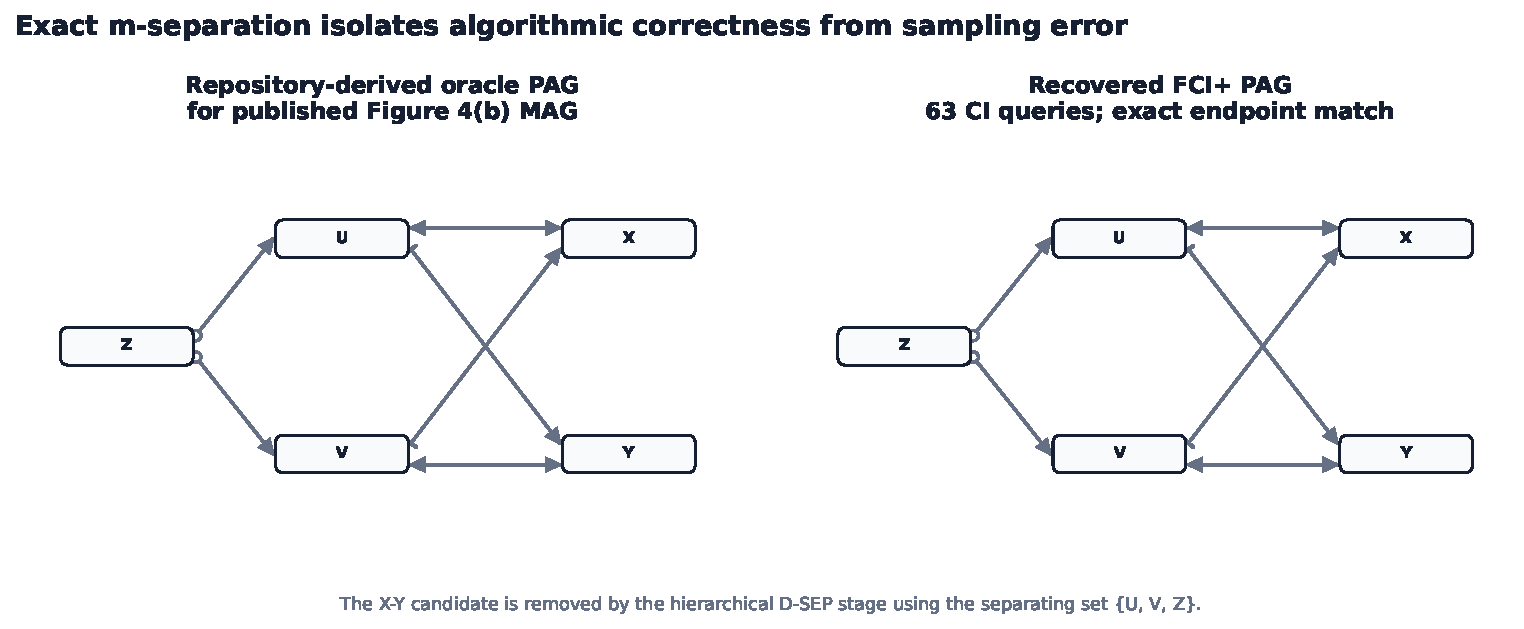
\includegraphics[width=\textwidth]{figure4_validation.pdf}
\caption{Exact-oracle validation on the central Figure~4(b) example. The
source-grounded facts are the six MAG edges and the exhibited separator
\(\{U,V,Z\}\); the endpoint-complete comparison target is independently
derived in the repository. Paper-aligned FCI needs 102 oracle queries,
\FCIplus{} 63; both recover the target exactly.}
\label{fig:figure4}
\end{figure}

\subsection{Finite-sample known-truth benchmark}

On a seeded latent linear SEM over the same reference graph, at
\(N = 5{,}000\) \FCIplus{} returns an extra \(X \leftrightarrow Y\)
(exact-edge F1 0.923) while standard FCI recovers the exact PAG; at
\(N = 50{,}000\) both are exact --- a reproducible fixture, not a universal
threshold.

Across the 15 cases (\cref{tab:executed-software-benchmark}, first three
rows), the robust profile improves the mean skeleton and
endpoint scores at about 2.04 times the CI cost of paper \FCIplus{} --- not
proof of universal dominance, but a check that the STAR stability gain
reported below is not bought by discarding structure, and a warning that
fewer CI tests do not imply better accuracy: the algorithms take different
logical routes after the initial skeleton and make different errors. Oracle tests support pipeline correctness under exact CI
information; finite-sample results remain limited by CI-test error and
tuning.

\begin{table}[!t]
\caption{Executed known-truth comparison: means over 15 completed runs
(five latent-SEM families, three seeds each, 2,500 observations).}
\label{tab:executed-software-benchmark}
\centering
\begin{tabularx}{\textwidth}{p{0.24\textwidth}rrrrrY}
\toprule
Method (version) & Skeleton F1 & Exact F1 & Semantic F1 &
Endpoint acc. & Seconds & Logical CI \\
\midrule
Local FCI paper (0.1.0) & 0.977 & 0.532 & 0.943 & 0.737 & 0.020 & 449.7 \\
Local \FCIplus{} paper (0.1.0) & 0.979 & 0.536 & 0.951 & 0.744 & 0.009 & 197.1 \\
Local \FCIplus{} robust (0.1.0) & 0.985 & 0.730 & 0.985 & 0.840 & 0.018 & 401.9 \\
causal-learn FCI (0.1.4.7) & 0.979 & 0.536 & 0.951 & 0.744 & 0.009 & not exposed \\
R \code{pcalg} \FCIplus{} \mbox{2.7-12} & 0.979 & 0.536 & 0.951 & 0.744 & 0.500 & not exposed \\
\bottomrule
\end{tabularx}
\end{table}

\subsection{Comparison with established software}

The equality of the aggregate local paper-\FCIplus{}, causal-learn, and
\code{pcalg} scores in \cref{tab:executed-software-benchmark} is useful
differential evidence, not an equivalence proof: local and causal-learn
timings are in-process whereas the R timing includes process startup, and
\code{pcalg::fciPlus} exposes no identical degree-bound control. The executed layer thus supports C3: matched aggregate behaviour
where interfaces overlap, alongside the integration gap documented in
\cref{sec:background}.

\subsection{Observed randomized-arm outcomes}

The small-minus-regular kindergarten contrast is 13.90 points
(school-cluster 95\% interval 5.21 to 22.07), while the regular-with-aide
contrast is 0.31 points (\(-7.40\) to 7.38). At grade 3 among observed
students the small-class contrast remains 11.69 points (3.74 to 19.38) and
the aide contrast 0.51 (\(-5.70\) to 7.22). Observation rates show no
precise arm difference: small minus regular is \(+1.54\) percentage points
(\(-1.73\) to 4.56), aide minus regular \(-2.05\) (\(-5.35\) to 1.41)
(\cref{tab:arm-summary}).

\begin{table}[!t]
\caption{Observed outcome summaries by kindergarten class arm. Intervals use
1,000 kindergarten-school bootstrap samples. Grade-3 summaries condition on
both scores being observed; kindergarten summaries also exclude missing
score components, so both are design-supported observed-outcome comparisons
rather than a fully reconstructed intention-to-treat estimand.}
\label{tab:arm-summary}
\centering
\begin{tabular}{llrrr}
\toprule
Outcome & Arm & \(n\) & Estimate & 95\% interval \\
\midrule
\multirow{3}{*}{Kindergarten score}
 & Regular & 2,005 & 918.04 & 908.78 to 927.05 \\
 & Regular + aide & 2,043 & 918.36 & 908.52 to 927.07 \\
 & Small & 1,738 & 931.94 & 922.70 to 940.12 \\
\addlinespace
\multirow{3}{*}{Grade-3 score}
 & Regular & 1,047 & 1246.74 & 1238.96 to 1254.01 \\
 & Regular + aide & 1,019 & 1247.25 & 1238.53 to 1255.48 \\
 & Small & 936 & 1258.43 & 1250.58 to 1266.17 \\
\addlinespace
\multirow{3}{*}{Grade-3 observed}
 & Regular & 2,194 & 47.72\% & 42.72\% to 52.14\% \\
 & Regular + aide & 2,231 & 45.67\% & 40.64\% to 50.39\% \\
 & Small & 1,900 & 49.26\% & 44.46\% to 53.77\% \\
\bottomrule
\end{tabular}
\end{table}

\subsection{Structure discovery across the three panels}

On the attrition panel the three implementations substantially agree at the
skeleton level (\cref{fig:pag-attrition}; costs and agreement in
\cref{tab:agreement-performance}). All three omit a direct
\code{K\_Class}--\code{Grade3\_Observed} adjacency, which appears in only
12--16\% of school bootstraps. By contrast,
\code{K\_Achievement}--\code{Grade3\_Observed} is adjacent in 100\% of
bootstrap fits for all three local profiles and the free-lunch/observation
adjacency is also stable: later availability is not independent of early
achievement and measured context. The three endpoint readings diverge:
standard FCI gives the impossible \emph{grade-3 observation
\(\rightarrow\) kindergarten achievement}; self-\FCIplus{} leaves a circle;
R-\FCIplus{} gives the temporally admissible direction. The R reading is
more plausible, but package identity cannot establish statistical
correctness. The attrition PAG does not prove a missingness mechanism; a
formal analysis would need an explicit estimand and further assumptions.

\begin{figure}[!t]
\centering
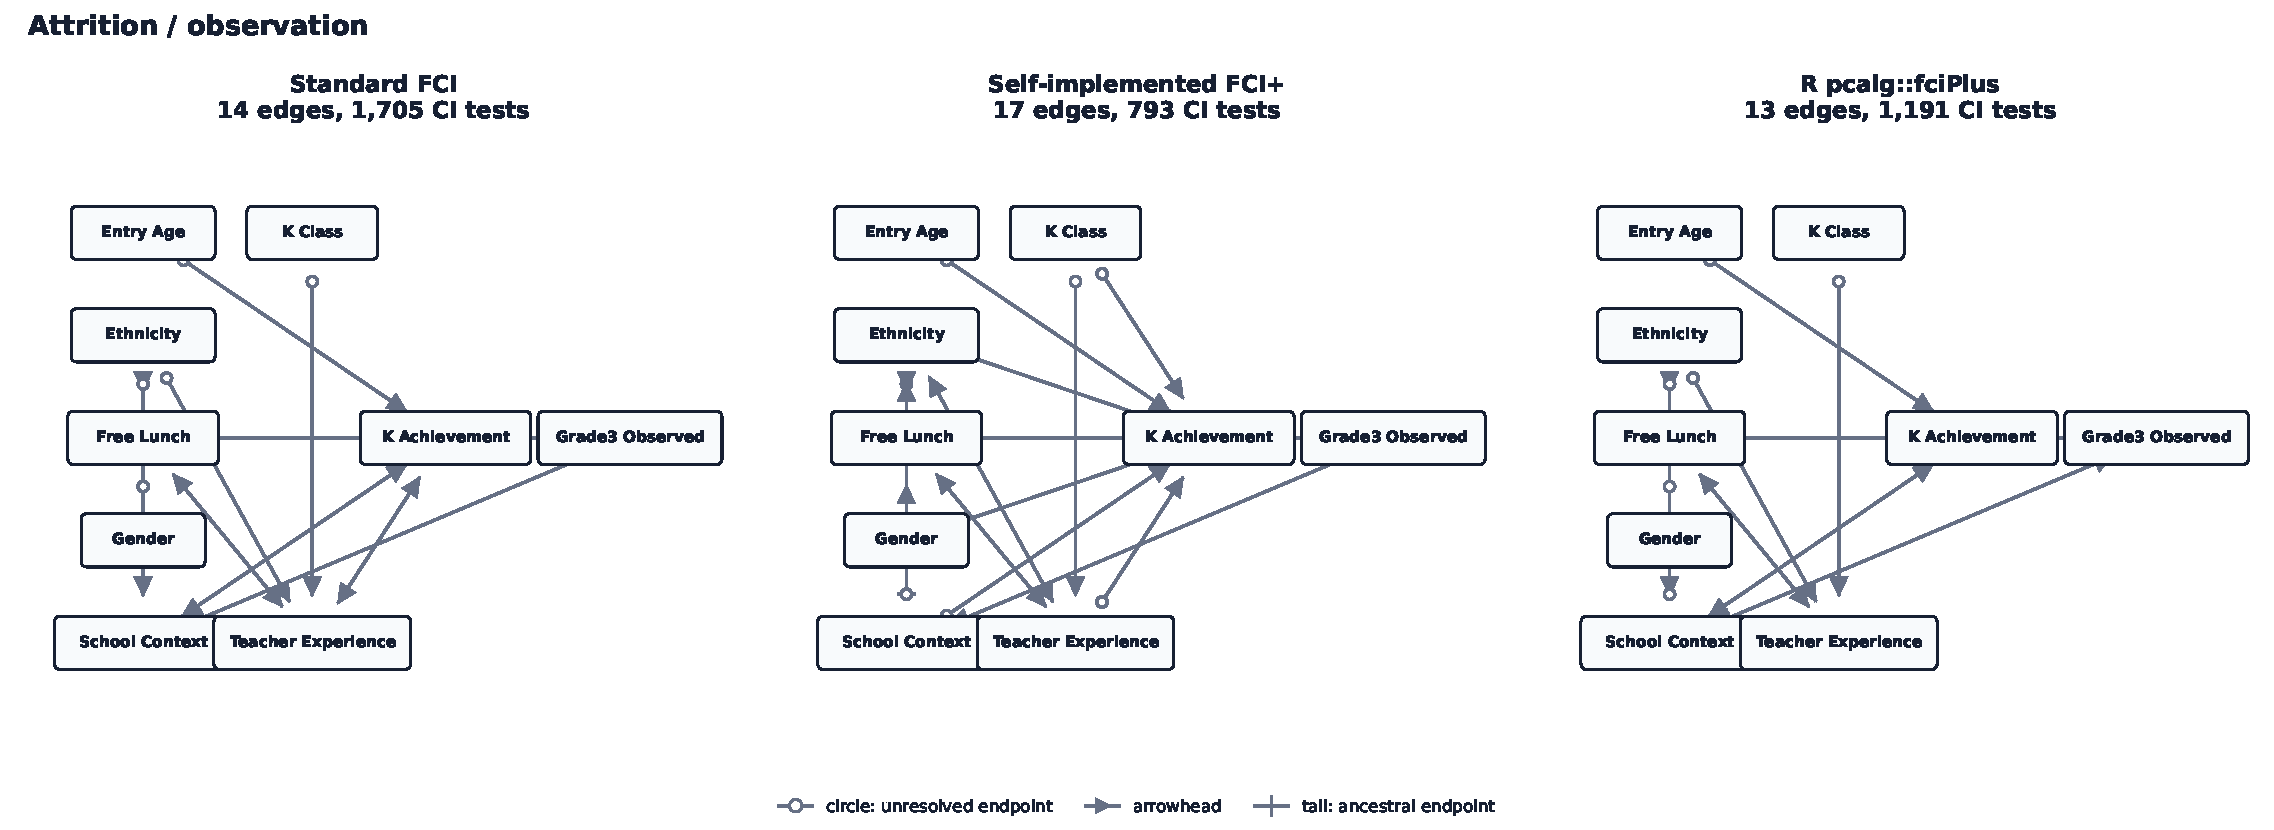
\includegraphics[width=\textwidth]{pag_attrition.pdf}
\caption{Three PAGs for the attrition/observation panel: self-implemented
FCI, self-implemented \FCIplus{}, and R \code{pcalg::fciPlus}. The skeletons
substantially overlap, while the achievement/observation endpoint differs
across implementations.}
\label{fig:pag-attrition}
\end{figure}

On the longitudinal panel all three implementations retain the
kindergarten/grade-3 achievement adjacency, present in all 100 bootstrap
samples for every local profile. No full-data PAG retains a direct
class-assignment/grade-3 adjacency once kindergarten achievement is
included, yet that adjacency reappears in 71\% of FCI, 79\% of paper
\FCIplus{}, and 80\% of robust-profile bootstrap fits --- a warning that
conservative orientation and order invariance do not remove
school-resampling sensitivity. Both \FCIplus{} implementations orient
grade-3 achievement toward kindergarten achievement, which is temporally
impossible if read causally, while standard FCI leaves that endpoint
unresolved. Agreement between implementations is not sufficient to override
chronology: both may replicate the same finite-sample CI pattern under
complete-case selection.

Removing kindergarten achievement changes the result: all three algorithms
return the same 10-edge PAG --- not merely the same skeleton --- including
\(\mathit{K\_Class} \leftrightarrow \mathit{Grade3\_Achievement}\)
(\cref{fig:pag-focused}), an adjacency appearing in 92\%, 85\%, and 96\% of
FCI, paper, and robust bootstraps. Independent exact replication makes this
conditional-independence pattern more credible, but it does not make a
literal latent-confounding reading credible: kindergarten class assignment
was randomized, while the focused panel conditions on grade-3 outcomes
being observed and omits early post-assignment achievement. Selection on
observation, school-level dependence, omitted post-randomization variables,
and CI-test error can all produce arrowheads at both endpoints.

\begin{figure}[!t]
\centering
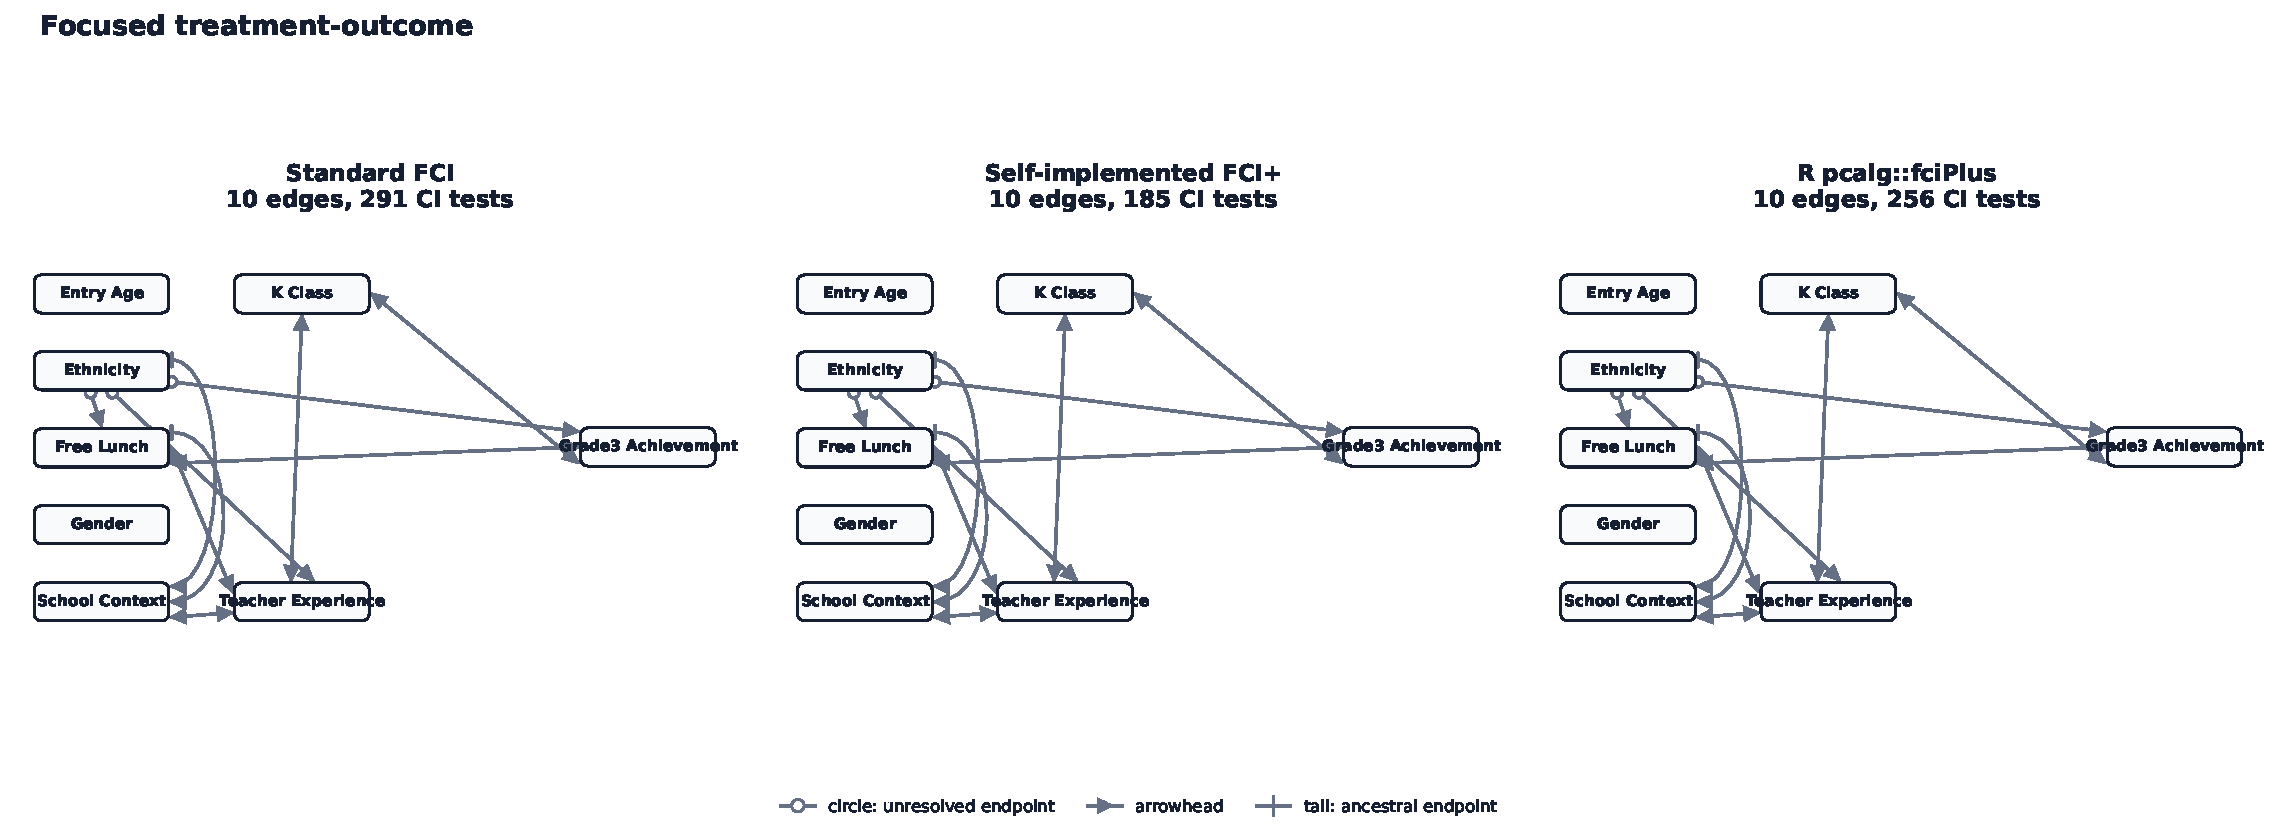
\includegraphics[width=\textwidth]{pag_focused_treatment.pdf}
\caption{PAGs for the focused complete-case panel. All three algorithms
recover the exact same 10-edge skeleton and endpoint pattern, including the
bidirected class-assignment/grade-3 edge.}
\label{fig:pag-focused}
\end{figure}

The sensitivity result is decisive (\cref{fig:sensitivity}): the focused
adjacency is robust to the tested bin count and degree bound but not to the
CI threshold: at \(\alpha = 0.01\) no local configuration retains it, while
at \(\alpha = 0.05\) the paper profiles retain a bidirected mark for every
tested \(k\) and the robust endpoint keeps circles. The stricter threshold
demands more evidence against independence, so removal indicates the edge
rests on relatively weak conditional-dependence evidence rather than an
invariant feature.

\begin{figure}[!t]
\centering
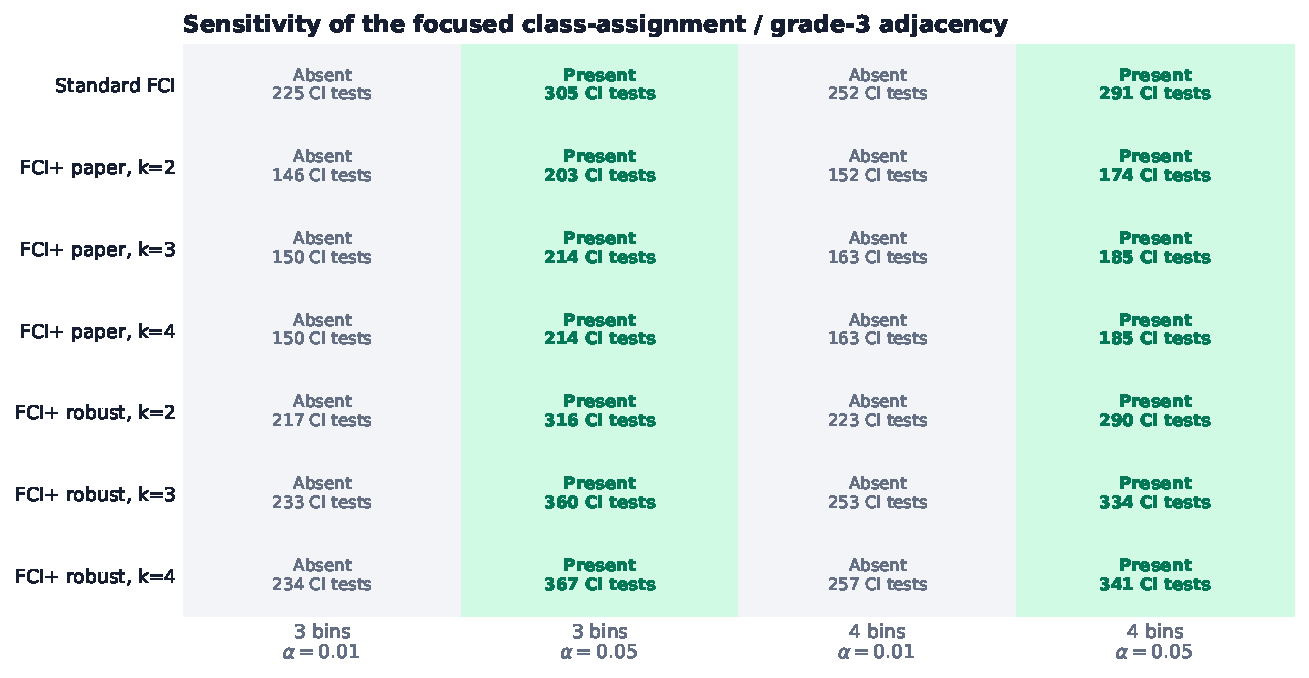
\includegraphics[width=0.88\textwidth]{star_sensitivity.pdf}
\caption{Focused treatment-outcome sensitivity. The adjacency appears at
\(\alpha = 0.05\) and disappears at \(\alpha = 0.01\), regardless of whether
three or four quantile bins or \(k = 2, 3, 4\) is used for \FCIplus{}.}
\label{fig:sensitivity}
\end{figure}

\subsection{Robust application profile, agreement, and cost}

The robust profile is a finite-sample decision layer, not a fourth paper
implementation. It returns 17, 12, and 10 edges on the three panels, with
target relations
\(\mathit{K\_Achievement} \circ\!-\!\circ \mathit{Grade3\_Observed}\),
\(\mathit{K\_Achievement} \circ\!-\!\circ \mathit{Grade3\_Achievement}\),
and \(\mathit{K\_Class} \circ\!-\!\circ \mathit{Grade3\_Achievement}\). It
retains the target skeleton information without the chronology reversal or
the bidirected over-interpretation.

In the cyclic-order audit, paper self-\FCIplus{} reproduces the exact
full-data PAG in 9 of 9 attrition, 5 of 9 longitudinal, and 6 of 8 focused
shifts, with one longitudinal temporal reversal; the R reference preserves
every panel skeleton while matching exact endpoints in 7 of 9, 6 of 9, and
6 of 8 shifts; robust self-\FCIplus{} returns the identical PAG in all 26
refits with no reversal. \Cref{tab:agreement-performance} summarises
agreement and search cost. Paper \FCIplus{} uses 46.5\%, 34.9\%, and 63.6\%
of the standard-FCI CI-test counts on the three panels (R reference:
69.9\%, 49.5\%, 88.0\%). Runtime is not language neutral, so CI-call counts
are the more interpretable comparison. Relative to paper self-\FCIplus{},
the robust profile uses 1.64 to 1.85 times as many CI calls, purchasing
stable deletion and invariant conservative endpoints rather than speed. In
summary, the robust profile returns the same full PAG for every tested order
with every target adjacency intact and no backward-in-time directed edge ---
at the price of under-orientation and extra CI work. Reliability has
improved; identifiability has not.

\begin{table}[!t]
\caption{Three-algorithm structural agreement (left) and search cost
(right). Endpoint rates use only adjacencies shared by the indicated pair;
time is the median of three full-data repetitions.}
\label{tab:agreement-performance}
\centering
\small
\begin{minipage}[t]{0.46\textwidth}
\centering
\begin{tabular}{llrr}
\toprule
Panel & Pair & Jaccard & Endpoints \\
\midrule
\multirow{3}{*}{Attr.}
 & FCI / self & 0.824 & 50.0\% \\
 & FCI / R & 0.929 & 61.5\% \\
 & self / R & 0.765 & 38.5\% \\
\addlinespace
\multirow{3}{*}{Long.}
 & FCI / self & 0.769 & 50.0\% \\
 & FCI / R & 0.833 & 70.0\% \\
 & self / R & 0.923 & 83.3\% \\
\addlinespace
\multirow{3}{*}{Focus.}
 & FCI / self & 1.000 & 100.0\% \\
 & FCI / R & 1.000 & 100.0\% \\
 & self / R & 1.000 & 100.0\% \\
\bottomrule
\end{tabular}
\end{minipage}
\hfill
\begin{minipage}[t]{0.50\textwidth}
\centering
\begin{tabular}{llrrr}
\toprule
Panel & Algorithm & Edges & CI & Sec. \\
\midrule
\multirow{4}{*}{Attr.}
 & FCI & 14 & 1,705 & 5.437 \\
 & self paper & 17 & 793 & 1.788 \\
 & self robust & 17 & 1,304 & 2.838 \\
 & R-\FCIplus{} & 13 & 1,191 & 10.394 \\
\addlinespace
\multirow{4}{*}{Long.}
 & FCI & 10 & 960 & 2.148 \\
 & self paper & 13 & 335 & 0.337 \\
 & self robust & 12 & 619 & 0.562 \\
 & R-\FCIplus{} & 12 & 475 & 1.650 \\
\addlinespace
\multirow{4}{*}{Focus.}
 & FCI & 10 & 291 & 0.322 \\
 & self paper & 10 & 185 & 0.159 \\
 & self robust & 10 & 334 & 0.247 \\
 & R-\FCIplus{} & 10 & 256 & 0.884 \\
\bottomrule
\end{tabular}
\end{minipage}
\end{table}

\section{Discussion}
\label{sec:interpretation}

\subsection{Evidence hierarchy}

An explicit hierarchy prevents a visually definite PAG mark from outranking
the experimental design. Tier 1: randomized assignment with the
school-cluster contrast, permitting a bounded causal statement for the
analysed observed outcome. Tier 2: an adjacency replicated across methods,
resamples, orders, and sensitivity settings --- a robust skeleton-level
claim with no magnitude or direction. Tier 3: a stable skeleton with circles
or endpoint disagreement, where adjacency is more credible than orientation.
Tier 4: an implementation-, order-, or chronology-sensitive endpoint ---
diagnostic evidence only. Tier 5: a threshold-sensitive or complete-case
exploratory pattern --- a hypothesis for external validation.

\subsection{What can and cannot be concluded}

The Tier-1 result --- the 13.90-point small-class contrast --- is consistent
with a beneficial early effect, but it is not an identified causal effect in
the post-assignment observed subset without assumptions about missing
outcomes, compliance, and the original randomization blocks. The aide
contrasts are close to zero at both time points: no evidence that an aide
reproduces the small-class advantage. The achievement--achievement and
achievement--observation adjacencies replicate across all fits and
bootstraps: a robust \emph{skeleton-level} relationship between early
performance, later performance, and later availability (Tier 2). The full-data attrition PAGs retain no
direct class-arm/observation adjacency and its bootstrap frequency is low:
concern about selective attrition is supported without a stable direct arm
effect on observation.

Conversely: no unique DAG is identified --- every PAG represents an
equivalence class --- and no effect magnitude comes from FCI. A bidirected
edge is not proof of a hidden confounder; in the focused panel it conflicts
with the known randomization unless selection or post-treatment conditioning
is considered. Temporal reversals are algorithm diagnostics, not credible
chronology. Implementation agreement is not proof: shared CI decisions and
rules can reproduce the same wrong endpoint. The 26 recorded shifts are a
finite audit, not a proof of order invariance; bootstrap frequency is not a
posterior probability. Absence is policy conditional: failure to retain an
edge under one node set, test, and threshold is not proof of zero effect.

\subsection{Limitations of the method}

FCI-family guarantees require faithfulness and correct CI decisions; the
threshold-sensitive focused edge demonstrates the practical consequence.
The true STAR-MAG degree is unobserved, so \(k=3\) is an analysis setting, not
a verified sparsity assumption. Discretisation enables G-square testing but
discards within-bin information and creates sparse conditional tables. The
row-wise CI test is not cluster-robust; school bootstrapping diagnoses
sensitivity to school composition but does not repair that mismatch. Finally,
version 0.1.0 and hand-authored oracle targets provide strong regression
evidence, not a formal correctness proof or exhaustive MAG-equivalence check.

A deterministic scaling audit (5 to 80 nodes; a directed chain and the
Figure~4(b) core with isolated variables added) recovers the exact target
skeleton in every run but yields an unexpected finding --- the query
advantage is not universal: \FCIplus{} wins on the five-node core (62 versus
101 queries) yet spends 5,162 versus 3,251 at 80 nodes, and 24,338 versus
12,638 on the 80-node chain --- consistent with a worst-case bound;
augmentation has a real cost when targeted D-SEP search offers little benefit.

\subsection{Limitations of the STAR study}

The longitudinal and focused panels condition on observed grade-3 scores and
may open selection paths. Kindergarten achievement is post-assignment:
including it may block part of the class-size pathway, while excluding it may
leave post-treatment dependence. Reporting both panels exposes this choice but
does not identify either model as correct. Original randomization blocks,
class switching, compliance, and school-specific procedures are not
reconstructed; the composite score also leaves subject-specific and subgroup
effects unexamined.

\section{Conclusion and Future Work}
\label{sec:conclusions}

All four objectives were achieved, with explicit scope qualifications.
\textbf{O1 was met}: the package implements source-located FCI and Algorithm~2
profiles with typed, auditable results. \textbf{O2 was met}: all three exact
targets were recovered, 367 tests pass, and the 15-run benchmark quantifies
finite-sample error. \textbf{O3 was met with interface limits}: matched
causal-learn and \code{pcalg} runs reproduce aggregate paper-profile scores,
although neither exposes every control or diagnostic. \textbf{O4 was met
within its structural scope}: the STAR workflow completed all planned
replication and stability audits, but it identifies neither a formal
intention-to-treat effect nor a unique causal graph.

The STAR evidence supports a 13.90-point observed kindergarten small-class
advantage, no comparable aide advantage, stable early--later achievement
structure, and selective later observation. The independently replicated
focused 10-edge PAG is nevertheless threshold-sensitive, and some endpoints
change with order or contradict chronology. Robust \FCIplus{} removes those
literal reversals by retaining circles, at 1.64--1.85 times the paper-profile
CI cost. Reliability improves; identifiability does not.

The hardest engineering work was translating ordered Possible-D-SEP pools and
Algorithm~2 hierarchy/revisit semantics into executable invariants, then
diagnosing finite-sample endpoint instability. Oracle-first validation,
separating algorithm from application, and committing every seed and artifact
worked well. Literal paper profiles did not provide sufficiently stable
real-data endpoints, so that failure is reported rather than silently
overridden with chronology. No method wins uniformly: paper \FCIplus{} is the
fidelity and query-efficiency subject, while robust \FCIplus{} is preferred for
this application under the declared audits.

The contribution is an auditable map of conditional-independence constraints
and modelling sensitivity, not a rediscovered STAR causal model. Next steps
are to reconstruct randomization strata for a formal intention-to-treat
analysis; add cluster-aware CI tests and endpoint-level stability summaries;
separate reading and mathematics; test temporal background knowledge as a
distinct analysis; and derive target PAGs with an exhaustive MAG-equivalence
oracle.

\paragraph{Reproduction.} The \code{run\_case\_study} module rebuilds the STAR
application with three benchmark repetitions, 100 discovery bootstraps, and
1,000 descriptive bootstraps; its refresh option re-executes the R reference.
Scripts under \code{reports/} regenerate every figure, the frozen
Figure~4(b) evidence, and the scaling audit. The committed
\code{STAR\_Students.tab.gz} has SHA-256
\code{2ffa578822eb30fcd6626fa7c5cc734a\brk 721fd05dd522403f0d643f89e891bac8}.%
\footnote{This document is the standalone final report; every number is
regenerated from committed artifacts by the listed scripts. Extended
per-stage evidence tables and complete source locators are kept in the
repository's full report, reports/fci\_plus\_star\_report.tex.}

\small
\bibliographystyle{plainnat}
\begin{thebibliography}{99}

\bibitem[Achilles et al.(2008)]{achilles2008star}
Achilles, C. M., Bain, H. P., Bellott, F., Boyd-Zaharias, J., Finn, J.,
Folger, J., Johnston, J., and Word, E. (2008).
Tennessee's Student Teacher Achievement Ratio (STAR) project.
Harvard Dataverse, V1. \url{https://doi.org/10.7910/DVN/SIWH9F}.

\bibitem[Claassen et al.(2013)]{claassen2013learning}
Claassen, T., Mooij, J. M., and Heskes, T. (2013).
Learning sparse causal models is not NP-hard.
In \textit{Proceedings of the 29th Conference on Uncertainty in Artificial
Intelligence}.

\bibitem[causal-learn developers(2026)]{causallearn2026}
causal-learn developers (2026).
\textit{FCI: Fast Causal Inference}. Official documentation, accessed
26 July 2026.

\bibitem[Glymour et al.(2019)]{glymour2019review}
Glymour, C., Zhang, K., and Spirtes, P. (2019).
Review of causal discovery methods based on graphical models.
\textit{Frontiers in Genetics}, 10, 524.

\bibitem[Kalisch et al.(2012)]{kalisch2012pcalg}
Kalisch, M., M{\"a}chler, M., Colombo, D., Maathuis, M. H., and
B{\"u}hlmann, P. (2012).
Causal inference using graphical models with the R package pcalg.
\textit{Journal of Statistical Software}, 47(11), 1--26.

\bibitem[Krueger(1999)]{krueger1999experimental}
Krueger, A. B. (1999).
Experimental estimates of education production functions.
\textit{The Quarterly Journal of Economics}, 114(2), 497--532.

\bibitem[Pearl(2009)]{pearl2009causality}
Pearl, J. (2009).
\textit{Causality: Models, Reasoning, and Inference}, second edition.
Cambridge University Press.

\bibitem[Richardson and Spirtes(2002)]{richardson2002ancestral}
Richardson, T. S. and Spirtes, P. (2002).
Ancestral graph Markov models.
\textit{The Annals of Statistics}, 30(4), 962--1030.

\bibitem[Spirtes et al.(2000)]{spirtes2000causation}
Spirtes, P., Glymour, C., and Scheines, R. (2000).
\textit{Causation, Prediction, and Search}, second edition. MIT Press.

\bibitem[Tetrad Project(2026)]{tetrad2026}
Tetrad Project (2026).
\textit{Tetrad 7.6.10 release and FCI source}. Official CMU repository,
accessed 26 July 2026.

\bibitem[Word et al.(1990)]{word1990star}
Word, E., Johnston, J., Bain, H. P., Fulton, B. D., Zaharias, J. B.,
Achilles, C. M., Lintz, M. N., Folger, J., and Breda, C. (1990).
\textit{Student/Teacher Achievement Ratio (STAR): Tennessee's K--3 Class
Size Study. Final Summary Report 1985--1990}.
Tennessee State Department of Education.

\bibitem[Zhang(2008)]{zhang2008completeness}
Zhang, J. (2008).
On the completeness of orientation rules for causal discovery in the
presence of latent confounders and selection bias.
\textit{Artificial Intelligence}, 172(16--17), 1873--1896.

\end{thebibliography}

\end{document}
